\documentclass[11pt,a4paper]{article}
\usepackage[T1]{fontenc}
\usepackage{mathptmx}
\usepackage{textcomp}
\usepackage[margin=2cm]{geometry}
\usepackage{amsmath,amssymb}
\usepackage{graphicx}
\usepackage{booktabs}
\usepackage[hidelinks]{hyperref}
\usepackage{enumitem}
\usepackage{caption}
\usepackage{float}
\captionsetup{font=small,labelfont=bf}
\setlist{itemsep=1pt,topsep=3pt}
\setlength{\parskip}{4pt}
\setlength{\parindent}{0pt}

\hypersetup{pdftitle={Assignment 1: Polynomial Regression - BT2024013},pdfauthor={Yash Sultania}}
\newcommand{\repo}{\url{https://github.com/yashh-s/ML_Assignment1}}

\title{\vspace{-1.2cm}\textbf{Assignment 1: Polynomial Regression}}
\author{Yash Sultania \quad (BT2024013)}
\date{}

\begin{document}
\maketitle
\vspace{-1.0cm}

\textbf{Final models.}
\textbf{var1:} degree 5 polynomial fitted with Lasso (L1), CV MSE $=0.313$, CV $R^2=0.969$.
\textbf{var2:} degree 11 polynomial fitted with Ridge (L2), CV MSE $=0.254$, CV $R^2=0.995$.\\
\textbf{Code:} \repo

%==========================================================
\section{Approach}

\textbf{Polynomial features.} For $d$ inputs, a degree-$D$ polynomial contains every term
$x_1^{a_1}x_2^{a_2}\cdots x_d^{a_d}$ with $a_1+\dots+a_d\le D$. There are $\binom{d+D}{D}$ such terms
(including the constant), e.g.\ 462 terms for var1 at $D=5$ and 364 for var2 at $D=11$.
Putting these terms as columns gives a matrix $\Phi$, and the model $\hat y=\Phi\mathbf w$ is linear in $\mathbf w$,
so it can be fitted with least squares exactly like in Lecture 6.

\textbf{Choosing the degree: 5-fold cross-validation (Lecture 7).}
The test labels are hidden, so every choice is made using only the training data. The 1000 training rows are split
into 5 blocks; the model is trained on 4 blocks and its MSE is measured on the 5th, and this is repeated so each block is used for
validation once. The CV MSE is the average over the 5 folds (I repeated this with 2--3 different random splits and averaged).
The model with the lowest CV MSE is chosen and then refitted on all 1000 rows to predict the test set.

\textbf{Three ways to fit the weights.} For each degree I compared:
\begin{itemize}
\item \textbf{Plain least squares (L6):} $\min_\mathbf{w}\|\mathbf{y}-\Phi\mathbf{w}\|^2$
\item \textbf{Ridge (L7):} $\min_\mathbf{w}\|\mathbf{y}-\Phi\mathbf{w}\|^2+\lambda\|\mathbf{w}\|_2^2$, \;i.e.\ $\hat{\mathbf{w}}=(\Phi^T\Phi+\lambda I)^{-1}\Phi^T\mathbf{y}$
\item \textbf{Lasso (L8):} $\min_\mathbf{w}\frac{1}{2N}\|\mathbf{y}-\Phi\mathbf{w}\|^2+\alpha\|\mathbf{w}\|_1$, \;which sets many weights exactly to zero
\end{itemize}
The penalty strength ($\lambda$ or $\alpha$) was also chosen by CV, from about 30 values on a log scale.
Degrees searched: 1--10 for var1 and 1--20 for var2 (the limits given in the problem).
For very high degrees $\Phi^T\Phi$ is close to singular, so instead of inverting it directly I used a numerically stable
least-squares solver (SVD), which gives the same answer. Lasso was fitted with scikit-learn.

\textbf{Data check.} No missing values or duplicates. All inputs lie in $[-1,1]$ and many values are exactly $\pm1$
(they look clipped). In var1, the test set has noticeably more of these edge values than the training set (Fig.~\ref{fig:eda}).
Polynomials are usually least accurate at the edges, so I expect var1's real test error to be slightly higher than its CV error.
As a check, I recomputed the CV error giving more weight to edge points (to match the test set's mix), and it picked the same models.

\begin{figure}[H]
\centering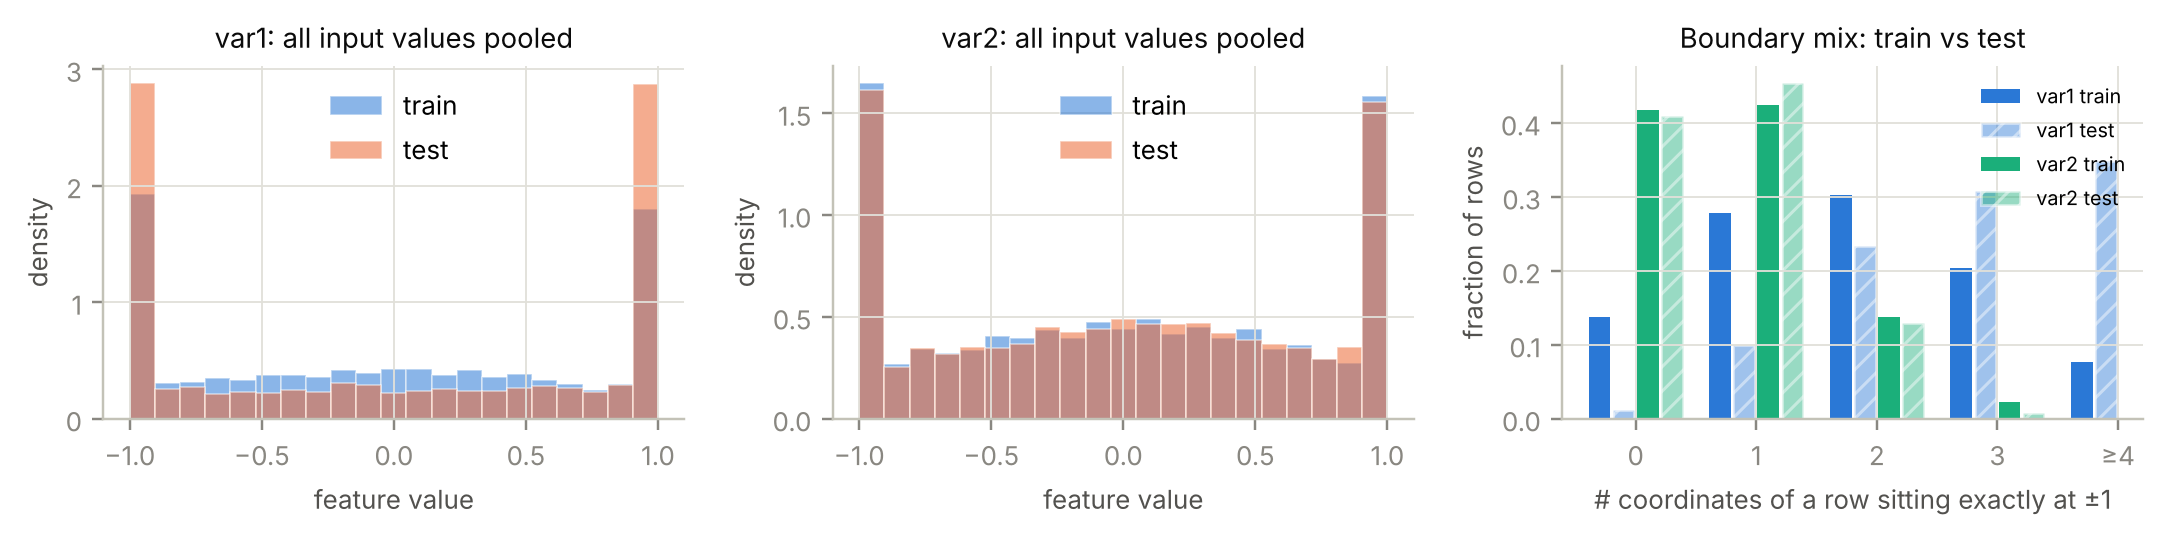
\includegraphics[width=\linewidth]{../figures/eda.png}
\vspace{-14pt}
\caption{Input values in train vs test. The spikes at $\pm1$ are clipped values. Right: how many coordinates of each row sit exactly on $\pm1$; var1's test set (hatched blue) has many more such rows.}
\label{fig:eda}
\end{figure}

%==========================================================
\section{var1 (6 inputs, degree $\le 10$)}

\begin{figure}[H]
\centering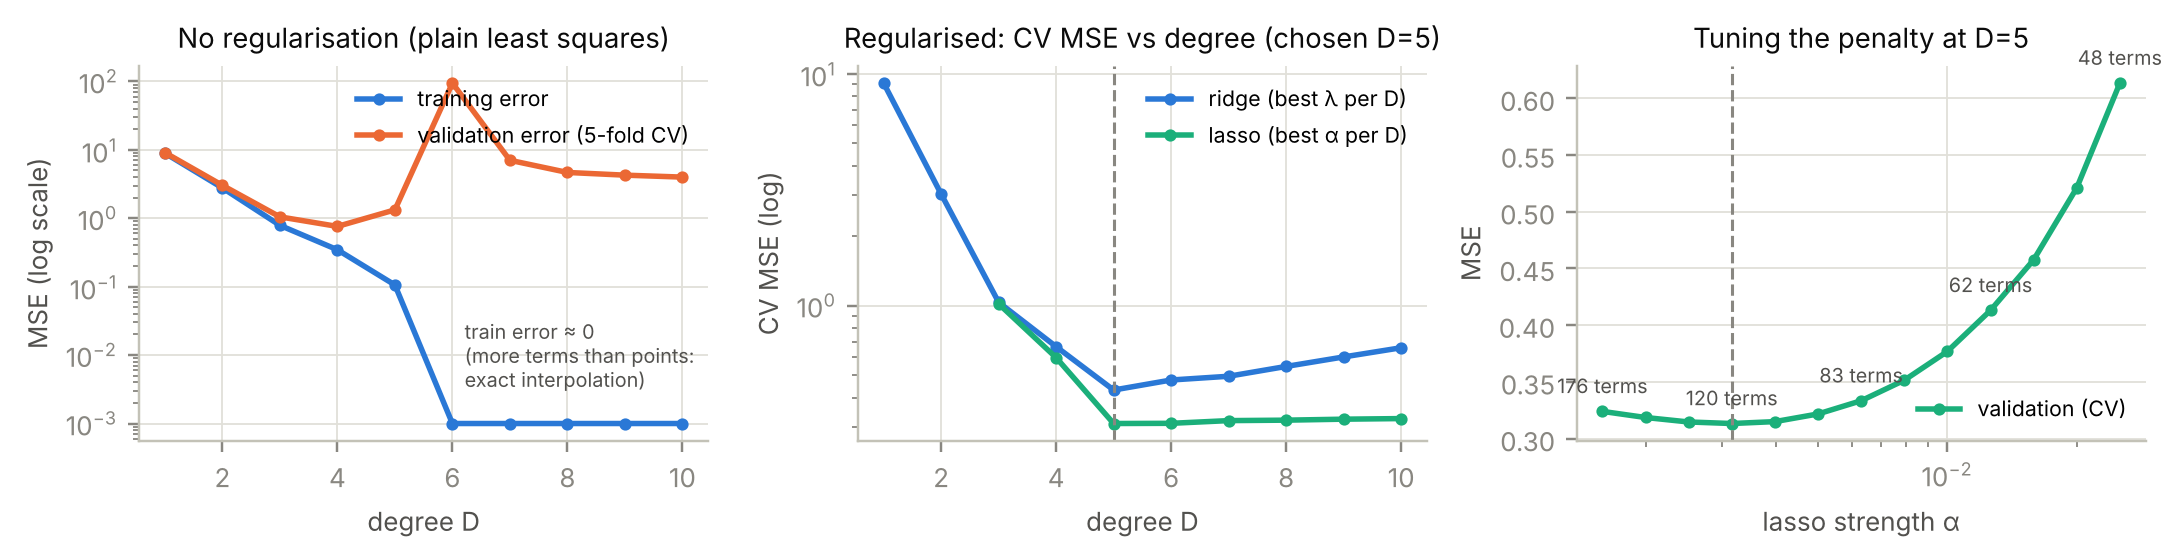
\includegraphics[width=\linewidth]{../figures/cv_var1.png}
\vspace{-14pt}
\caption{var1. \textbf{Left:} plain least squares. Validation error is lowest at $D=4$ and jumps at $D=6$, where there are 924 terms but only 800 training rows per fold, so the model fits the training data exactly (training error $\approx0$) and fails on new data. \textbf{Centre:} best CV error for each degree with Ridge and Lasso. \textbf{Right:} CV error vs Lasso strength $\alpha$ at $D=5$, with the number of non-zero terms.}
\label{fig:cv1}
\end{figure}

\begin{table}[H]
\centering\small
\begin{tabular}{lcccc}
\toprule
Method & best $D$ & penalty & CV MSE & non-zero terms\\
\midrule
Plain least squares & 4 & -- & 0.760 & 210\\
Ridge & 5 & $\lambda=3.16$ & 0.433 & 462\\
\textbf{Lasso (chosen)} & \textbf{5} & $\boldsymbol{\alpha\approx0.003}$ & \textbf{0.313} & \textbf{115}\\
\bottomrule
\end{tabular}
\caption{var1 comparison (5-fold CV). Predicting the mean of $y$ every time would give MSE $\approx 10.2$.}
\end{table}

\textbf{Why degree 5.} Without regularisation we see the usual underfit/overfit pattern (Fig.~\ref{fig:cv1}, left):
low degrees underfit, and from $D=5$ there are too many coefficients for 800 rows, so plain least squares is best at $D=4$.
With regularisation the overfitting is controlled, and $D=5$ becomes clearly better than $D=4$ (0.31 vs 0.60 with Lasso).
Going higher does not help: with Lasso, $D=6$ scores 0.311, the same as $D=5$, and higher degrees are slightly worse.
Since $D=5$ and $D=6$ are tied, I chose the simpler model, $D=5$.

\textbf{Why Lasso.} Lasso keeps only 115 of the 462 terms and sets the rest to exactly zero, and it beats Ridge by a wide margin
(0.31 vs 0.43). This means only some of the polynomial terms actually matter, which is the case Lecture 8 recommends L1 for.
Ridge has to give a small weight to every term, including the useless ones, and those small weights partly fit noise.
The most important terms Lasso found include $x_1x_5$, $x_2^3x_3$ and $x_3x_6$.

\textbf{Choosing $\alpha$.} If $\alpha$ is too large, Lasso removes terms that are needed (with 48 terms left the CV MSE is 0.61);
if it is too small, useless terms come back. The best value was $\alpha\approx0.003$ (about 115 terms).

%==========================================================
\section{var2 (3 inputs, degree $\le 20$)}

\begin{figure}[H]
\centering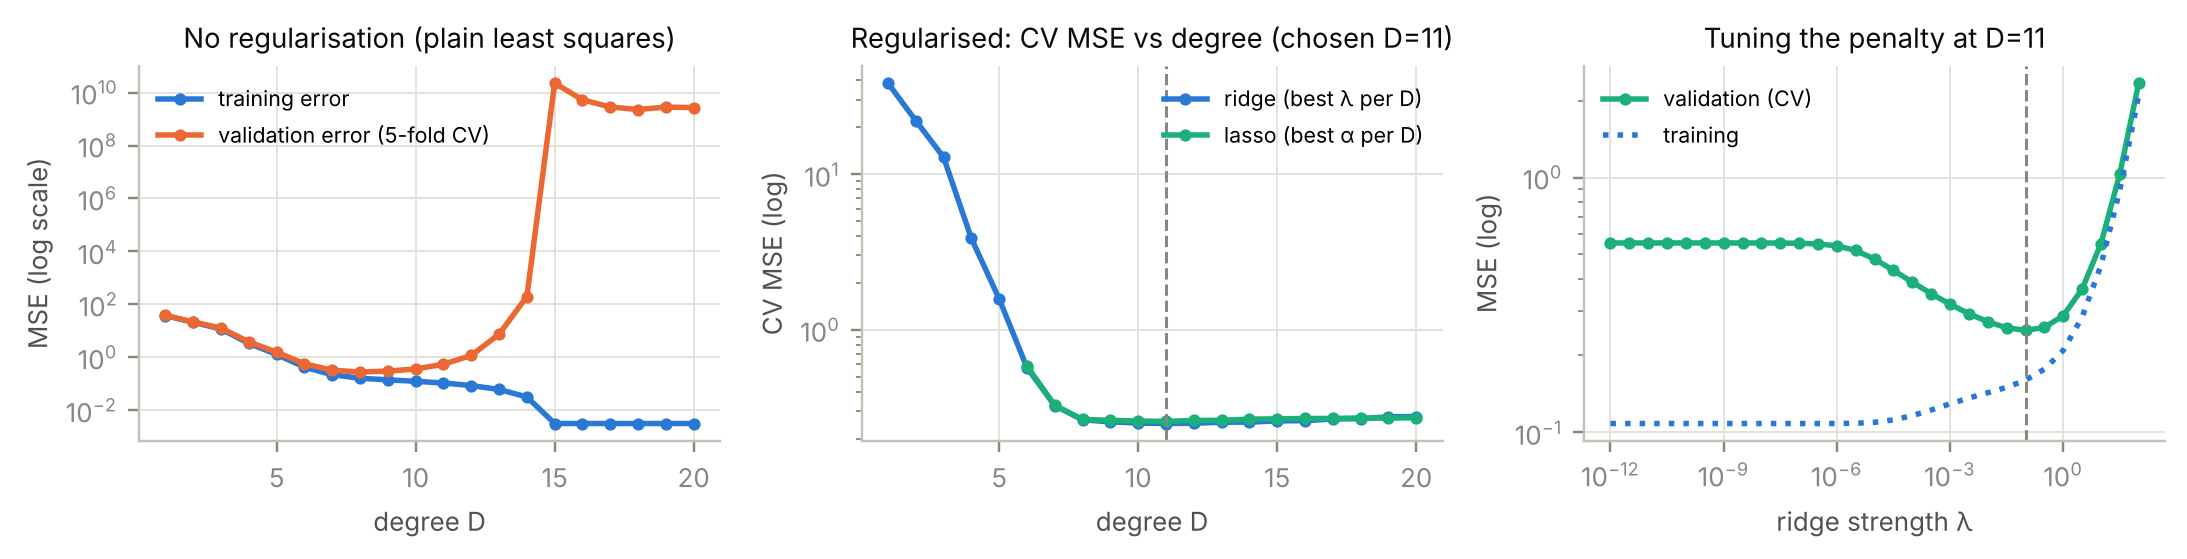
\includegraphics[width=\linewidth]{../figures/cv_var2.png}
\vspace{-14pt}
\caption{var2. \textbf{Left:} plain least squares is best at $D=8$; beyond $D\approx12$ the validation error explodes (overfitting). \textbf{Centre:} with Ridge or Lasso the CV error stays flat at $\approx0.25$ from $D\approx9$ onwards. \textbf{Right:} Ridge strength at $D=11$: a tiny $\lambda$ overfits, a large $\lambda$ underfits.}
\label{fig:cv2}
\end{figure}

\begin{table}[H]
\centering\small
\begin{tabular}{lcccc}
\toprule
Method & best $D$ & penalty & CV MSE & CV $R^2$\\
\midrule
Plain least squares & 8 & -- & 0.281 & 0.994\\
Lasso & 11 & $\alpha=10^{-4}$ & 0.259 & 0.995\\
\textbf{Ridge (chosen)} & \textbf{11} & $\boldsymbol{\lambda=0.1}$ & \textbf{0.254} & \textbf{0.995}\\
\bottomrule
\end{tabular}
\caption{var2 comparison (5-fold CV). Predicting the mean of $y$ every time would give MSE $\approx 49.7$.}
\end{table}

\textbf{Why degree 11.} var2 needs a high degree: the CV error drops from 38.2 at $D=1$ to about 0.26 at $D=8$.
Plain least squares cannot go further because it starts overfitting, but with Ridge every degree from 9 to 14 gives
almost the same CV error (0.251--0.257). $D=11$ had the lowest value. Because these degrees are so close, I checked
that the choice doesn't really matter: test predictions from the best Ridge models at $D=9,10,12,14$ differ from the $D=11$
predictions by only about 0.05--0.07 (RMS), much smaller than the typical error of $\approx0.5$.

\textbf{Why Ridge here.} Unlike var1, Lasso does not help: Ridge, Lasso and plain least squares all end up at about 0.25--0.28.
This looks like the noise level of the data, which no model can remove. I chose Ridge because it scored slightly best and has a
simple closed-form solution.

%==========================================================
\section{Checks}

\begin{figure}[H]
\centering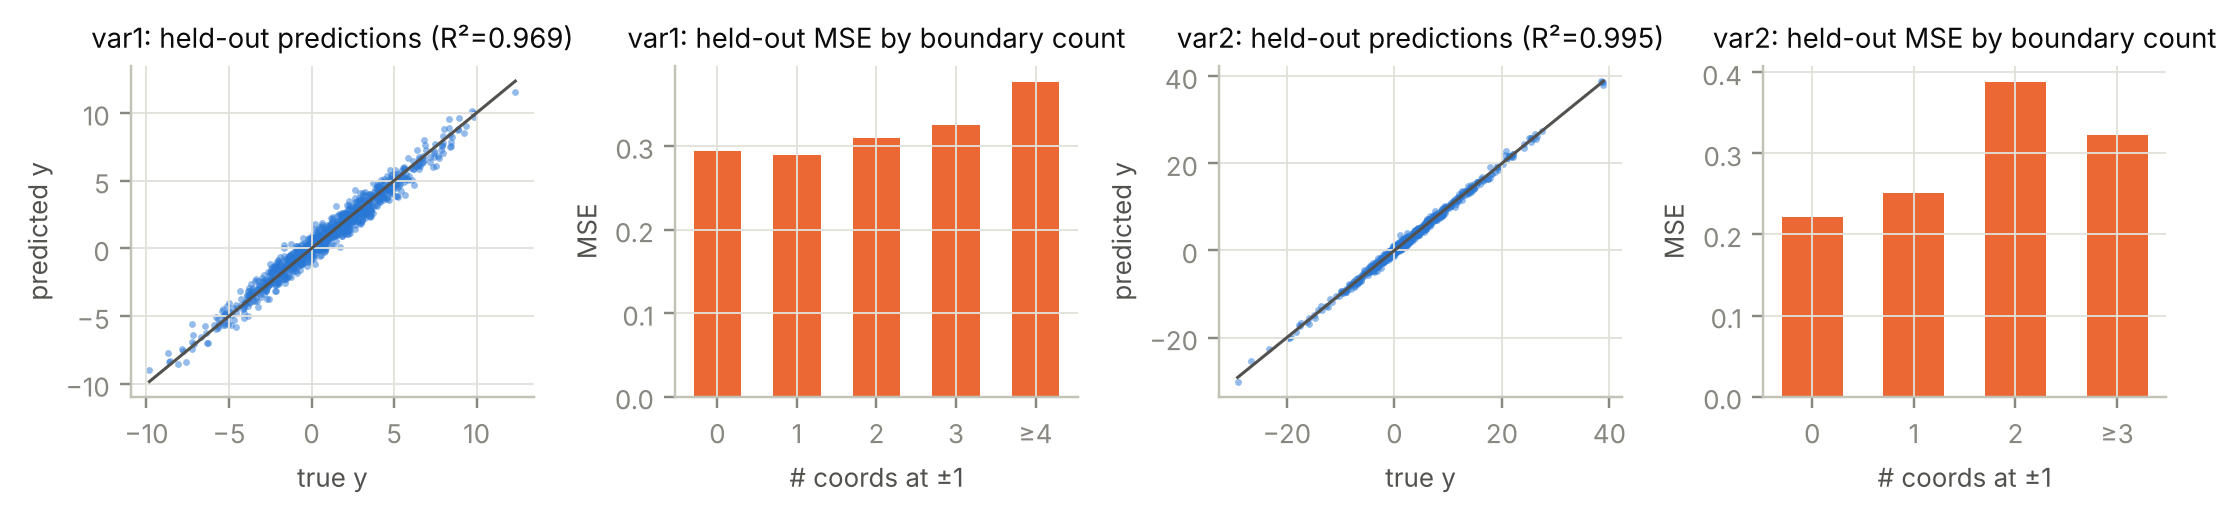
\includegraphics[width=\linewidth]{../figures/residuals.png}
\vspace{-14pt}
\caption{Predictions on held-out folds vs the true values, and held-out MSE grouped by how many coordinates sit on $\pm1$.}
\label{fig:resid}
\end{figure}

\begin{itemize}
\item \textbf{No overfitting:} training $R^2$ (0.977 for var1, 0.997 for var2) is only slightly higher than the CV $R^2$ (0.969 and 0.995).
An overfit model would show a big gap, like plain least squares at high degree does in Figs.~\ref{fig:cv1} and~\ref{fig:cv2}.
\item \textbf{Held-out predictions} lie close to the $y=\hat y$ line for both problems (Fig.~\ref{fig:resid}).
\item \textbf{Edge points:} for var1 the error grows from about 0.29 for rows with no coordinate on $\pm1$ to about 0.38 for rows with 4 or more.
Since the var1 test set has many of these rows, I expect its test MSE to be a little above 0.31 (roughly 0.33).
\item \textbf{Elastic Net (L8)}, a mix of L1 and L2, was also tried for var1 and did not beat plain Lasso (CV MSE 0.32--0.36).
\end{itemize}

%==========================================================
\section{Code}
Repository: \repo.\;
\texttt{polyreg.py} builds the polynomial features and the least-squares/Ridge solver;
\texttt{cv\_ridge.py} and \texttt{cv\_lasso.py} run the cross-validation searches;
\texttt{final\_model.py} fits the chosen models on all training data and writes the two prediction files;
\texttt{self\_check.py} holds out 20\% of the training data and reports MSE and $R^2$;
\texttt{make\_figures.py} makes the figures in this report.

\end{document}
